%% Master article: comparison of quantised small language models for
%% grammar-constrained command parsing on a Raspberry Pi 5.
%% Elsevier CAS double-column template (cas-dc, els-cas-templates 2024).
%% Build: pdflatex main -> bibtex main -> pdflatex main -> pdflatex main
%% (or upload this folder, including thumbnails/ and figures/, to Overleaf).

\documentclass[a4paper,fleqn]{cas-dc}

\usepackage[authoryear]{natbib}
%% Local builds without the STIX/Charis fonts fall back to Latin Modern (vector) instead of
%% bitmap Computer Modern; on Overleaf, where STIX is installed, this line does nothing.
\IfFileExists{stix.sty}{}{\usepackage{lmodern}}
\usepackage{xurl}
%% Long model names (e.g. Llama-3.2-1B-Instruct) cannot hyphenate; allow a little extra stretch.
\setlength{\emergencystretch}{2em}
\usepackage{listings}
\lstset{basicstyle=\ttfamily\scriptsize,breaklines=true,columns=fullflexible,
        frame=none,aboveskip=4pt,belowskip=4pt}

\newcommand{\pp}{\,pp}
\newcommand{\QF}{Q4\_K\_M}
\newcommand{\QE}{Q8\_0}

%% The template always prints an "ORCID(s):" footnote line. It is suppressed until the
%% authors' ORCID iDs are added (\author[1]{Name}[orcid=0000-0000-0000-0000]); then delete it.
\renewcommand{\printorcid}{}

\begin{document}
\let\WriteBookmarks\relax
\def\floatpagepagefraction{1}
\def\textpagefraction{.001}

\shorttitle{Quantised small language models for command parsing on a Raspberry Pi 5}
\shortauthors{T. Kahia and B. Khaldi}

\title [mode = title]{Quantised small language models for grammar-constrained command
parsing on a Raspberry Pi 5: an accuracy--efficiency comparison}

\author[1]{Tayeb Kahia}
% \cormark[1]   % PLACEHOLDER: mark the corresponding author
\ead{<email-author-1>}
\credit{Conceptualization, Methodology, Software, Investigation, Data curation, Formal analysis,
Visualization, Writing -- original draft}

\author[1]{Belkacem Khaldi}
% \cormark[1]   % PLACEHOLDER: mark the corresponding author
\ead{<email-author-2>}
\credit{Conceptualization, Methodology, Supervision, Writing -- review \& editing}

\affiliation[1]{organization={\'Ecole Sup\'erieure en Informatique -- 08 Mai 1945},
            city={Sidi Bel Abb\`es},
            country={Algeria}}

\cortext[1]{Corresponding author: <to be confirmed>}

\begin{abstract}
A drone that must keep working without a network has to parse spoken commands on its own
processor. We compare three instruction-tuned small language models, SmolLM2-360M,
Qwen2.5-0.5B and Llama-3.2-1B, fine-tuned with low-rank adaptation to map transcripts of
drone-swarm commands to a fixed JSON schema, quantised to Q8\_0 and Q4\_K\_M, and decoded under a
bounded grammar by \texttt{llama.cpp} on the CPU of a Raspberry Pi~5. A fourth model of matched
size, H2O-Danube3-500M, controls for model family. On a 200-item golden test set of recorded
commands, scored on reference transcripts, Qwen2.5-0.5B at Q4\_K\_M reaches an exact match of
0.935 and Llama-3.2-1B 0.910, a difference that is not significant (exact McNemar $p = 0.0625$);
both exceed SmolLM2-360M (0.760). At matched size, family alone separates Qwen2.5-0.5B from
H2O-Danube3-500M by 6.5 percentage points ($p = 0.0023$). The accuracy cost of the deployment
pipeline, from the fp16 model to the quantised artefact under the grammar, lies within
$\pm$1.5 points and is not significant, and removing the grammar produces one malformed output in
3,540 decodes. On the cooled board Qwen2.5-0.5B decodes at 27.93 tokens/s; without active
cooling every trial throttled and throughput fell to 18.13 tokens/s, below the 20 tokens/s
floor. A selection rule that applies the deployment constraints first selects Qwen2.5-0.5B at
Q4\_K\_M only after re-baselining the latency budget: its end-to-end latency (3,122~ms at the
95th percentile) exceeds the 2,500~ms budget, and no configuration meets the false-command target on out-of-domain input
($\leq$~0.05; measured 0.19--0.39) or the safe-failure target.
\end{abstract}

\begin{highlights}
\item Three fine-tuned small language models parse drone commands on a Raspberry Pi 5
\item A 0.5B model scores 0.935 against 0.910 for a 1.2B model, a non-significant gap
\item At matched size, model family alone changes exact match by 6.5 points
\item Without its grammar, the parser emitted one malformed output in 3,540 decodes
\item Qwen2.5-0.5B falls below the 20 tokens/s throughput floor without active cooling
\end{highlights}

\begin{keywords}
Small language models \sep Post-training quantisation \sep Grammar-constrained decoding \sep
Edge inference \sep Spoken command parsing \sep Unmanned aerial vehicles
\end{keywords}

\maketitle

% =============================================================================
\section{Introduction}
\label{sec:intro}

Language models are now a common interface between human instructions and robot actions,
including aerial ones~\citep{saycan2022,chatgptrobotics2024,typefly2024}. Most such systems call
a large model on a remote server. An aircraft that should keep working when the link drops
cannot rely on that server, so its command parser has to run on the onboard computer, which on a
small platform is a CPU-only single-board computer. Benchmarks of quantised language models on
such boards find that they reliably serve models of up to about 1.5 billion
parameters~\citep{sbc2025}. Whether a model that small is accurate enough for a given task is a
separate question, and it has to be answered on the task.

Command parsing adds a requirement that general benchmarks do not capture. The parser's output is
read by a controller, not by a person, and a controller cannot act on a command that is right in
intent but malformed in syntax. Structural validity is therefore a precondition rather than one
component of accuracy. In a preliminary zero-shot test on the target board, Qwen2.5-0.5B under an
early grammar repeated drone identifiers for the command ``swarm land'' until the token cap
truncated the output; the truncated output failed to parse, and the landing was lost.
Grammar-constrained decoding makes such failures unreachable by masking every token that would
violate a grammar~\citep{willard2023,koo2024}, provided that the grammar itself is bounded.

The components of this problem have been studied separately. Benchmarks on single-board computers
time models without scoring a task~\citep{sbc2025}. Quantisation studies score general-purpose
benchmarks with an unconstrained decoder, mostly at larger scales~\citep{kurtic2025,kurt2026,slmquant}.
Studies of constrained decoding evaluate models that were not fine-tuned to the target
format~\citep{geng2023,tam2024}. Choosing a model to deploy on a board requires task accuracy
under the deployed runtime and grammar, measured together with latency, throughput and memory on
that board.

This article reports such a comparison for a voice interface that commands a swarm of five
simulated drones. The system around the parser, including its speech front end, safety layers and
formation control, is described in a companion paper~\citep{companion}; here we address model
selection. The contributions are:
\begin{itemize}
\item A comparison of three fine-tuned small language models of 0.36--1.24~B parameters at two
  GGUF quantisation levels under a bounded grammar. It scores accuracy and abstention with paired
  statistical tests and times latency, throughput and memory on a Raspberry Pi~5.
\item A parameter-matched control showing that, at about 0.5~B parameters, model family alone
  changes exact match by 6.5 percentage points.
\item A measurement of the accuracy cost of the full deployment pipeline, from the fp16 model to
  the quantised artefact under the grammar, and a grammar ablation that measures what the grammar
  adds once a model has been fine-tuned to the format.
\item Evidence that the thermal state of the board decides whether the selected model meets the
  throughput floor,
  and a selection rule that applies the deployment constraints first and reports its own failure,
  including two abstention targets that no configuration meets.
\end{itemize}

Section~\ref{sec:related} reviews the closest work. Section~\ref{sec:methods} describes the task,
models and protocol, Section~\ref{sec:results} reports the measurements,
Section~\ref{sec:discussion} discusses them, and Section~\ref{sec:conclusion} concludes.

% =============================================================================
\section{Related work}
\label{sec:related}

\paragraph{Language models as robot command interfaces.} SayCan weights a language model's
proposals by the value functions of a robot's pretrained skills~\citep{saycan2022}. \citet{chatgptrobotics2024} use ChatGPT, served remotely, to produce robot code under human
supervision, and advise against giving such tools full control of the robotics pipeline.
TypeFly drives a single drone with GPT-4 through a compact plan language and keeps response time
below 1.5~s on its benchmark~\citep{typefly2024}. For swarms, CommandSwarm generates behaviour
trees with open models of 6.7--14~B parameters at 4-bit precision, gated by a
parser~\citep{commandswarm2026}, and LLM2Swarm is mainly conceptual, with a preliminary test of
TinyLlama on a Raspberry Pi~5~\citep{llm2swarm2024}. These systems rely on remote or multi-billion
parameter models, and none compares small models for on-board parsing under a latency budget.

\paragraph{Inference on single-board computers and quantisation.} \citet{sbc2025} benchmark 25
quantised models on three single-board computers under two runtimes. They find that models of up
to about 1.5~B parameters are served reliably and that the runtime alone changed throughput by up
to four times on one board. They report throughput and resource use, not task
accuracy. Post-training quantisation methods reduce the memory footprint of language
models~\citep{gptq}, and AWQ lists on-device deployment among its motivations~\citep{awq}. Their cost is evaluated as perplexity and accuracy on
general-purpose suites: for FP8, INT8 and INT4 formats on models of 1.5 to 405~B
parameters~\citep{kurtic2025}, for the \texttt{llama.cpp}
formats on Llama-3.1-8B-Instruct together with CPU throughput~\citep{kurt2026}, and for small
models on generic benchmarks~\citep{slmquant}. None of these studies scores a structured-output
task under a constrained decoder.

\paragraph{Grammar-constrained decoding.} Constrained decoding restricts, at every step, the tokens
a model may emit to those that keep the output inside a formal language, so that structural
validity holds by construction~\citep{willard2023,koo2024}. \citet{geng2023} apply grammars to
structured NLP tasks without fine-tuning. The literature also documents costs:
constraints distort the model's distribution over grammatical outputs~\citep{park2024}, and format
restrictions lower accuracy on reasoning tasks while matching or improving it on classification
tasks~\citep{tam2024}. These studies evaluate models that were not fine-tuned to the target format,
so what a grammar adds after fine-tuning is not reported.

\paragraph{Intent and slot corpora.} Mapping an utterance to an intent and its slots is an
established formulation of spoken-language understanding~\citep{qin2021}. SLURP and MASSIVE cover
assistant domains~\citep{slurp2020,massive}, and the Snips platform parses commands on embedded
hardware with a classical pattern-and-tagger pipeline rather than a language
model~\citep{snips2018}. We found no public corpus for swarm commands.

\paragraph{Gap.} No study we reviewed scores fine-tuned language models below 1.5~B parameters on a
command-parsing task under a grammar while timing the same quantised artefacts on a single-board
computer. This article fills that gap for one task and one device, and adds a family control, a
deployment-pipeline delta and a grammar ablation to the comparison.

% =============================================================================
\section{Methods}
\label{sec:methods}

\subsection{Task, command schema and grammar}
\label{sec:schema}

An operator speaks an English command to a swarm of five drones; a speech recogniser
(\texttt{whisper.cpp}, commit 52a939a, with the \texttt{tiny.en} model~\citep{whisper,whispercpp}) transcribes it,
and the parser maps the transcript to a single-line JSON command. Ten intents cover the vocabulary:
\texttt{formation}, \texttt{move}, \texttt{altitude}, \texttt{takeoff}, \texttt{land},
\texttt{hover}, \texttt{abort}, \texttt{rotate}, \texttt{set\_param} and \texttt{unknown}, the last
being the schema's only provision for an utterance that is not a supported command. Keys follow a
fixed order and absent slots are omitted, for example:
\begin{lstlisting}
{"intent":"formation","shape":"circle","radius":5.0}
{"intent":"move","dir":"north","dist":10.0}
{"intent":"altitude","z":4.0,"ids":[1,2]}
\end{lstlisting}
Omitting absent slots shortens the decode: over the 200 golden labels a command averages 16.0
tokens under the Qwen2.5 tokeniser, against 19.6 if each intent's absent slots were emitted as
nulls.

The schema is enforced by a context-free grammar in the GBNF formalism of
\texttt{llama.cpp}~\citep{llamacpp}, with one alternative per intent and enumerated shapes and
directions. Every rule is bounded. A number has at most three integer digits and one decimal, and
an identifier list holds at most five identifiers in $0$--$4$; the second bound removes the
repetition loop described in Section~\ref{sec:intro}. The grammar's language is therefore finite;
its longest string has 90 characters, so the 96-token decoding cap cannot truncate a command
before it closes. Numeric ranges are not expressible in GBNF and are checked by a downstream
validator~\citep{companion}.

\subsection{Dataset}
\label{sec:dataset}

The corpus is built label first: each target command is written before the sentences that express
it, and paraphrases are generated from 120 template families. Splits are assigned by family
(96/12/12 for training, validation and synthetic test), so every in-domain test item comes from
families held out from training. The training split has 1,940 pairs. In 872 of them the
transcript was replaced by the recogniser's output on synthesised speech, mixed with noise at 20,
10 or 5~dB signal-to-noise ratio, so that the parser sees recognition errors in training. The
\texttt{unknown} intent is taught by 81 pairs: 20 assistant-style queries, 21 requests for
capabilities the schema lacks and 40 near-misses that contain a command word.

Three test sets are used. The \emph{synthetic test set} has 240 pairs from the 12 held-out
families. The \emph{golden test set} has 200 commands read aloud by the first author in a quiet room,
drawn from the same 12 families; they cover all ten intents through 12 command patterns of 10--22
items each. The \emph{out-of-domain set} has 150 inputs whose reference is \texttt{unknown}:
assistant-style queries, unsupported requests, truncated fragments, and 12 recogniser outputs on
noise and silence. A 240-pair validation set selects checkpoints. Every accuracy figure in this
article takes the reference transcript as input. The recogniser's word error rate on the golden
speaker is 23.1\% (95\% CI 20.3--25.9) for the recogniser alone without its domain prompt, and
23.3\% through the deployed pipeline, where accuracy from audio is reported in the companion
paper~\citep{companion}.

\subsection{Models and fine-tuning}
\label{sec:models}

Three instruction-tuned models span the range in which single-board computers are practical:
SmolLM2-360M-Instruct~\citep{smollm2} with 362~M parameters, Qwen2.5-0.5B-Instruct~\citep{qwen25}
with 494~M, and Llama-3.2-1B-Instruct~\citep{llama32} with 1,236~M. Because each comes
from a different family, size and family are confounded among them. A fourth model,
H2O-Danube3-500M-Chat (514~M)~\citep{danube3}, lies within 4.0\% of Qwen2.5-0.5B in size and is
included as a family control, not as a deployment candidate.

All four were fine-tuned with the same LoRA recipe~\citep{lora}: rank 16, $\alpha = 32$, dropout
0.05, adapters on every attention and feed-forward projection, AdamW~\citep{adamw} with learning
rate $2\times10^{-4}$, cosine schedule and warm-up ratio 0.03, three epochs, effective batch size
32, sequence length 256, loss on the completion tokens only, fp16 precision on two T4 GPUs
(which lack native bf16, although the checkpoints are released in bf16), and
seed 42, with \texttt{peft} 0.19.1, \texttt{transformers} 5.0.0 and PyTorch 2.10.0 (CUDA 12.8)
in the session that trained the three candidates; the software image of the control's session was
not recorded. The checkpoint with the highest validation exact match was kept. The system prompt is
the single line ``You are a drone swarm command parser. Output only JSON matching schema.'', with
the transcript as the user turn. H2O-Danube3-500M's chat template has no system role, so its
system prompt was folded into the user turn, and it was trained in a separate session. Under the
three-epoch budget, validation exact match was unchanged between the second and third epochs only
for Llama-3.2-1B; it was still rising for the other three (Qwen2.5-0.5B by 0.008, SmolLM2-360M by
0.025 and H2O-Danube3-500M by 0.038), so no model is shown to have converged.

\subsection{Quantisation and evaluation surfaces}
\label{sec:surfaces}

The adapters were merged, converted to GGUF at fp16, and quantised with \texttt{llama-quantize}
to \QE{} and \QF{}~\citep{llamacpp}, giving six deployable artefacts. Accuracy is measured on two
surfaces. The \emph{reference surface} is the fine-tuned fp16 model decoded by
\texttt{transformers} without a grammar. The \emph{deployed surface} is a quantised artefact
decoded by \texttt{llama.cpp} (build b10863, commit 88ada91c) under the grammar, with a 96-token cap and one
sequence at a time. Decoding is greedy on both. Their difference is the accuracy cost of the
deployment pipeline as a whole, not of weight precision alone: precision, runtime, grammar and
decoding settings change together, and for Llama-3.2-1B the checkpoint as well, because its
validation exact match tied between epochs two and three. The grammar term is separated by the
ablation of Section~\ref{sec:res-ablation}.

A mismatch between the chat template used in training and the one applied at inference raises no
error and degrades accuracy silently. We therefore compared, over ten fixed prompts, both the
rendered text and the token identifiers produced by the training tokeniser and by
\texttt{llama.cpp}. The three deployment candidates pass on all ten. H2O-Danube3-500M renders
identical text but segments the word ``drone'' differently, so a quantised artefact of it would
not be the model that was trained; it is reported on the reference surface only.

Because greedy decoding is deterministic, accuracy was scored on a workstation; for the selected
configuration the outputs on the workstation and on the Raspberry~Pi~5 were identical for all 200
golden items. All timing was measured on the board.

\subsection{Hardware and timing protocol}
\label{sec:timing}

The target is a Raspberry Pi~5 with 8~GB of memory and four Cortex-A76 cores; core 0 is
reserved for the audio frame loop. \texttt{llama.cpp} runs on the other three cores with three
threads under the \texttt{performance} governor (2.4~GHz). Swap is disabled, one model is resident
at a time, and the page cache is dropped before each configuration loads. Each \QF{} configuration
is warmed up for ten minutes and then timed over 60 scored trials on a fixed sample of golden-set
transcripts; the
\QE{} artefacts were not timed. The run of record was made with an active cooler. An earlier run
under the same protocol without the cooler is reported for comparison. The server's prompt cache
was enabled during timing, so prefill figures are those of a cached prefix. Peak resident memory
of the language-model process was sampled every 20~ms, and the board's throttle flag was recorded
on every trial.

\subsection{Metrics}
\label{sec:metrics}

Exact match (EM) compares canonical forms of the prediction and the reference: key order fixed,
absent slots omitted, numbers rounded to one decimal, identifier lists sorted and deduplicated,
whitespace removed. Intent F1 is macro-averaged over intents; slot F1 is micro-averaged over
(key, value) pairs. Schema validity is the fraction of outputs that parse as a conforming command.
The safe-failure rate is, among wrong outputs, the fraction whose dispatched action is
\texttt{unknown} or \texttt{hover}. The false-command rate is, on the out-of-domain set, the
fraction of inputs whose dispatched action is anything other than \texttt{unknown}. Throughput is
decode tokens summed over decode time summed. Percentiles use the nearest-rank rule; p50 and p95
denote the 50th and 95th percentiles.

\subsection{Statistical analysis}
\label{sec:stats}

Every configuration decodes the same items deterministically, so predictions are paired and
McNemar's test~\citep{mcnemar1947} applies: the exact binomial test below 25 discordant pairs and
the continuity-corrected chi-square from 25 upwards. Two confirmatory families of three
comparisons were fixed before the results: model against model at \QF{}, and \QE{} against \QF{}
within each model, both on the golden test set, each Bonferroni-corrected~\citep{dunn1961} to
$\alpha = 0.0167$. Two comparisons added after the results are labelled exploratory: each fp16
reference against its quantised artefacts (six pairs, $\alpha = 0.0083$), and the family control
($\alpha = 0.05$). Each exact-match figure on the golden set is also given a 95\% percentile
bootstrap interval over items (10,000 replicates, fixed seed). Overlapping intervals do not
contradict a significant paired test: each interval describes one score, whereas the paired test
uses only the items on which two configurations disagree. The 200 golden items are paraphrases
of 12 patterns and are not independent, so the intervals are narrower, and the $p$-values smaller,
than they would be for independent items.

\subsection{Deployment targets and selection rule}
\label{sec:targets}

The targets were fixed with the schema, before any result existed: EM $\geq$~0.85 and intent F1
$\geq$~0.90 on the golden test set; prefill p95 $\leq$~250~ms and decode p95 $\leq$~1,100~ms, which
combine to a language-model allowance of 1,350~ms; a throughput floor of 20~tokens/s, which
follows from a 22-token decode allowance within 1,100~ms; end-to-end p95 $\leq$~2,500~ms from the
end of speech; peak memory $\leq$~2.5~GiB for the full stack; throttled trials $\leq$~5\%; a
safe-failure rate $\geq$~0.70; and a false-command rate $\leq$~0.05. The selection rule deploys the
configuration with the highest golden-set EM among those that satisfy the end-to-end budget and the
memory ceiling, breaking ties toward lower p95 latency. A partial measurement can show that a
configuration misses a constraint but not that it satisfies it. If no configuration satisfies both
constraints, each unmet constraint is re-baselined to the measured figure, and the re-baselining is
reported.

% =============================================================================
\section{Results}
\label{sec:results}

\subsection{Accuracy}
\label{sec:res-accuracy}

\begin{table*}[t]
\caption{Model comparison on the deployed surface (\texttt{llama.cpp}, grammar on). Accuracy on
the golden (200 items), synthetic (240) and out-of-domain (150) test sets, scored on reference
transcripts; on the out-of-domain set EM is the fraction of inputs answered with
\texttt{unknown}. Timing on the cooled Raspberry Pi~5, 60 trials per configuration, prefill and
decode combined; \QE{} was not timed. Mem.: peak resident memory of the language-model process.
95\% CI: percentile bootstrap over the golden items. Schema validity is 1.000 in every cell and
is omitted.}
\label{tab:comparison}
\footnotesize\setlength{\tabcolsep}{3pt}
\begin{tabular*}{\textwidth}{@{\extracolsep{\fill}}llccccccccc@{}}
\toprule
& & \multicolumn{4}{c}{Golden test set} & Synthetic & Out-of-domain & \multicolumn{3}{c}{Raspberry Pi 5} \\
\cmidrule(lr){3-6}\cmidrule(lr){9-11}
Model & Quant. & Intent F1 & Slot F1 & EM & 95\% CI & EM & EM & p50/p95 (ms) & tok/s & Mem. (GiB) \\
\midrule
SmolLM2-360M & \QE{} & 0.972 & 0.866 & 0.790 & [0.730, 0.845] & 0.812 & 0.607 & -- & -- & -- \\
             & \QF{} & 0.954 & 0.848 & 0.760 & [0.700, 0.815] & 0.812 & 0.660 & 475/894 & 40.63 & 0.55 \\
Qwen2.5-0.5B & \QE{} & 1.000 & 0.958 & 0.930 & [0.890, 0.965] & 0.958 & 0.733 & -- & -- & -- \\
             & \QF{} & 1.000 & 0.961 & \textbf{0.935} & [0.900, 0.965] & 0.954 & 0.747 & 647/1,072 & 27.93 & 0.68 \\
Llama-3.2-1B & \QE{} & 0.996 & 0.948 & 0.915 & [0.875, 0.950] & 0.963 & 0.800 & -- & -- & -- \\
             & \QF{} & 0.996 & 0.945 & 0.910 & [0.865, 0.945] & 0.958 & 0.813 & 1,351/2,282 & 14.53 & 1.63 \\
\bottomrule
\end{tabular*}
\end{table*}

Table~\ref{tab:comparison} reports the six deployed configurations. On the golden test set,
Qwen2.5-0.5B at \QF{} reaches an EM of 0.935 (95\% CI 0.900--0.965), Llama-3.2-1B 0.910
(0.865--0.945) and SmolLM2-360M 0.760 (0.700--0.815), below the 0.85 target, as is its 0.790 at
\QE{}. On the
synthetic and out-of-domain sets the ordering follows parameter count. Intent F1 on the golden set
exceeds 0.95 for every configuration and is 1.000 for Qwen2.5-0.5B. Of the 152 golden-set errors
across the six configurations, 133 (87.5\%) keep the reference intent and err in a parameter.
Schema validity is 1.000 in all 18 configuration--split cells. Prompted zero-shot at fp16, without
fine-tuning and without the grammar, none of the four models matches any of the 590 test items
(EM 0.000 on every split).

\begin{figure}
\centering
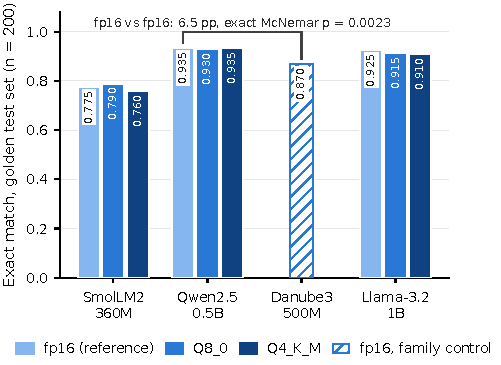
\includegraphics[width=\columnwidth]{figures/fig_em_bars.pdf}
\caption{Exact match on the golden test set by model and precision. fp16 bars are the fine-tuned
model on the reference surface (\texttt{transformers}, no grammar); \QE{} and \QF{} bars are the
deployed surface (\texttt{llama.cpp}, grammar on). H2O-Danube3-500M (hatched) has no deployed
artefact (Section~\ref{sec:surfaces}); the family contrast is drawn between the two fp16 bars.}
\label{fig:em}
\end{figure}

\subsection{Parameter-matched family control}
\label{sec:res-family}

Figure~\ref{fig:em} places the family control beside the three candidates. On the reference
surface, Qwen2.5-0.5B (494~M) reaches 0.935 (95\% CI 0.900--0.965) and H2O-Danube3-500M (514~M) 0.870
(0.820--0.915) on the golden set, a difference of 6.5 percentage points (pp) on 15 against 2
discordant items (exact McNemar $p = 0.0023$, exploratory), although the two intervals
overlap. The larger model of the pair is the less accurate on all three test
sets (synthetic 0.954 against 0.887; out-of-domain 0.727 against 0.720). Across the full size
range, from SmolLM2-360M (0.775) to Llama-3.2-1B (0.925), the reference-surface EM spans 15.0\pp{}
over a 3.4-fold difference in parameters, but the endpoints also differ in family.

\subsection{Accuracy cost of the deployment pipeline}
\label{sec:res-delta}

\begin{table}
\caption{Golden-set EM of each fp16 reference model and its deployed artefacts. $b$/$c$: items
only the reference / only the deployed artefact gets right; $p$: exact McNemar, exploratory
family of six ($\alpha = 0.0083$). Precision, runtime, grammar and decoding settings change
together.}
\label{tab:delta}
\footnotesize\setlength{\tabcolsep}{3pt}
\begin{tabular*}{\tblwidth}{@{\extracolsep{\fill}}llcccrc@{}}
\toprule
Model & Quant. & fp16 & Deployed & $\Delta$ (pp) & $b$/$c$ & $p$ \\
\midrule
SmolLM2-360M & \QE{} & 0.775 & 0.790 & $+1.5$ & 0/3 & 0.25 \\
             & \QF{} & 0.775 & 0.760 & $-1.5$ & 12/9 & 0.66 \\
Qwen2.5-0.5B & \QE{} & 0.935 & 0.930 & $-0.5$ & 1/0 & 1.00 \\
             & \QF{} & 0.935 & 0.935 & $0.0$ & 0/0 & 1.00 \\
Llama-3.2-1B & \QE{} & 0.925 & 0.915 & $-1.0$ & 2/0 & 0.50 \\
             & \QF{} & 0.925 & 0.910 & $-1.5$ & 3/0 & 0.25 \\
\bottomrule
\end{tabular*}
\end{table}

Table~\ref{tab:delta} compares each fp16 reference model with its deployed artefacts on the golden
set. The differences span $-1.5$ to $+1.5$\pp{}, no difference exceeds three items net, and none
reaches significance; the smallest $p$ is 0.25. SmolLM2-360M at \QE{} scores above its own fp16
reference.

\subsection{Grammar ablation}
\label{sec:res-ablation}

\begin{table}
\caption{Grammar ablation: the six deployed artefacts decode the same 590 items greedily with and
without the grammar; nothing else changes. EM is pooled by item over all models, precisions and
test sets.}
\label{tab:ablation}
\footnotesize\setlength{\tabcolsep}{3pt}
\begin{tabular*}{\tblwidth}{@{\extracolsep{\fill}}lcccc@{}}
\toprule
Condition & Decodes & Schema validity & Malformed & EM \\
\midrule
Grammar on  & 3,540 & 1.0000 & 0 & 0.8508 \\
Grammar off & 3,540 & 0.9997 & 1 & 0.8492 \\
\bottomrule
\end{tabular*}
\end{table}

Removing the grammar (Table~\ref{tab:ablation}) lowers schema validity from 1.0000 to 0.9997:
exactly one of 3,540 outputs is malformed. It came from Llama-3.2-1B at \QF{} on the
out-of-domain query ``what does lidar stand for'', which it answered with a sentence of prose.
Pooled EM falls from 0.8508 to 0.8492, a difference of 0.17\pp{}, or six decodes.

\subsection{Paired comparisons}
\label{sec:res-paired}

\begin{table}
\caption{McNemar tests on the golden test set (200 items). $b$/$c$: items only A / only B gets
right. Exact binomial test unless marked $^\dagger$ (continuity-corrected chi-square, 25 or more
discordant pairs).}
\label{tab:mcnemar}
\footnotesize\setlength{\tabcolsep}{3pt}
\begin{tabular*}{\tblwidth}{@{\extracolsep{\fill}}lcccl@{}}
\toprule
A vs B & EM A / EM B & $b$/$c$ & $p$ & Sig. \\
\midrule
\multicolumn{5}{@{}l}{\emph{Model vs model, \QF{} (confirmatory, $\alpha = 0.0167$)}} \\
Llama vs Qwen     & 0.910 / 0.935 & 0/5  & 0.0625 & no \\
Llama vs SmolLM2  & 0.910 / 0.760 & 34/4 & $2.5\times10^{-6\,\dagger}$ & yes \\
Qwen vs SmolLM2   & 0.935 / 0.760 & 38/3 & $1.1\times10^{-7\,\dagger}$ & yes \\
\multicolumn{5}{@{}l}{\emph{\QF{} vs \QE{} (confirmatory, $\alpha = 0.0167$)}} \\
Llama             & 0.910 / 0.915 & 0/1  & 1.00 & no \\
Qwen              & 0.935 / 0.930 & 1/0  & 1.00 & no \\
SmolLM2           & 0.760 / 0.790 & 8/14 & 0.29 & no \\
\multicolumn{5}{@{}l}{\emph{Family control, fp16 (exploratory, $\alpha = 0.05$)}} \\
Qwen vs Danube3   & 0.935 / 0.870 & 15/2 & 0.0023 & yes \\
\bottomrule
\end{tabular*}
\end{table}

Qwen2.5-0.5B and Llama-3.2-1B disagree on five golden items, all in Qwen2.5-0.5B's favour
(Table~\ref{tab:mcnemar}), $p = 0.0625$. Both models are separated from SmolLM2-360M. No
\QE{}--\QF{} pair differs significantly. On the synthetic set SmolLM2-360M scores 0.812 at both
precisions, and the two artefacts disagree on 24 items, split 12 to 12.

\subsection{Latency, throughput and memory}
\label{sec:res-latency}

\begin{figure}
\centering
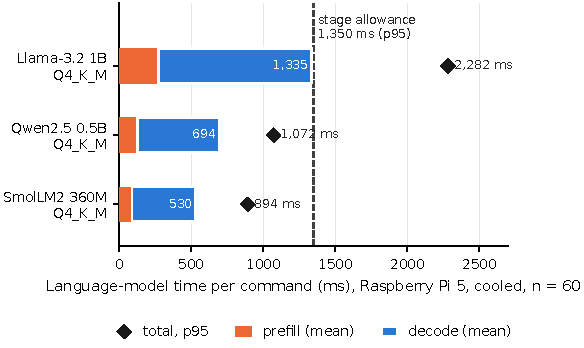
\includegraphics[width=\columnwidth]{figures/fig_latency_stack.pdf}
\caption{Language-model time per command at \QF{} on the cooled Raspberry Pi~5 (60 trials per
model, warm-up excluded). Bars stack mean prefill and mean decode, which add up to the mean total;
diamonds mark the measured p95 of the total, since percentiles of the two stages do not add. The
dashed line is the 1,350~ms language-model allowance, a p95 target. Prefill uses a cached prompt
prefix.}
\label{fig:latency}
\end{figure}

On the cooled board (Figure~\ref{fig:latency}), Qwen2.5-0.5B decodes at 27.93~tokens/s with a
combined prefill-and-decode p95 of 1,072~ms; SmolLM2-360M reaches 40.63~tokens/s and 894~ms, and
Llama-3.2-1B 14.53~tokens/s and 2,282~ms; Llama-3.2-1B misses the 20~tokens/s floor. Decode p95 is
1,033~ms, 785~ms and 1,842~ms respectively, against the 1,100~ms allowance, which Llama-3.2-1B
misses by 67\%. Prefill p95 is 328.8~ms for Qwen2.5-0.5B, which misses the 250~ms allowance (p50
38.5~ms; 8 of 60 trials above it), 241.4~ms for SmolLM2-360M and 457.5~ms for Llama-3.2-1B, whose
p50 of 267.7~ms already exceeds the allowance (34 of 60 trials above it). With a cached prefix,
Qwen2.5-0.5B has 278~ms to spare against the combined 1,350~ms allowance. Without the prompt cache,
as the deployed parser runs, its prefill p95 is 751~ms and its combined prefill-and-decode p95
1,658~ms, which misses the allowance~\citep{companion}. Peak resident
memory of the language-model process is 0.55, 0.68 and 1.63~GiB for the three models.

\subsection{Thermal state}
\label{sec:res-thermal}

\begin{figure}
\centering
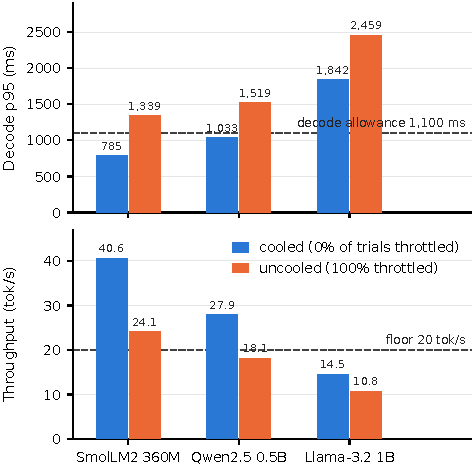
\includegraphics[width=\columnwidth]{figures/fig_thermal.pdf}
\caption{Decode p95 (top) and decode throughput (bottom) at \QF{}, with and without an active
cooler, on the same board, artefacts and protocol (60 trials each). Dashed lines: the 1,100~ms
decode allowance and the 20~tokens/s throughput floor.}
\label{fig:thermal}
\end{figure}

Without the active cooler, all 180 scored trials were throttled, against a limit of 5\%, with the
clock capped at 1.5~GHz
and peak temperatures of 90.6--91.1~$^\circ$C; with it, no trial was throttled and temperatures
stayed within 67.5--74.1~$^\circ$C (Figure~\ref{fig:thermal}). Cooling reduced decode p95 by
25.1\% to 41.3\% and raised throughput by 35.2\% to 68.5\%, the largest change being on the
smallest model. Qwen2.5-0.5B decodes at 18.13~tokens/s uncooled and 27.93~tokens/s cooled.

\subsection{Out-of-domain input and abstention}
\label{sec:res-ood}

\begin{figure}
\centering
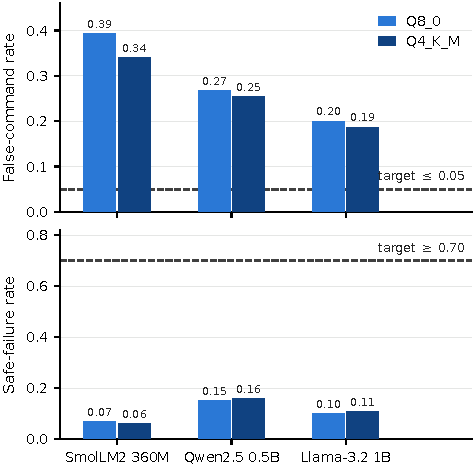
\includegraphics[width=\columnwidth]{figures/fig_ood.pdf}
\caption{Out-of-domain set (150 inputs, reference \texttt{unknown}). Top: false-command rate, the
fraction of inputs dispatched as anything other than \texttt{unknown}. Bottom: safe-failure rate,
the fraction of wrong outputs dispatched as \texttt{unknown} or \texttt{hover}. Dashed lines: the
deployment targets.}
\label{fig:ood}
\end{figure}

On the out-of-domain set (Figure~\ref{fig:ood}), the false-command rate ranges from 0.1867
(Llama-3.2-1B, \QF{}) to 0.3933 (SmolLM2-360M, \QE{}), against a target of $\leq$~0.05; the
configurations answer \texttt{unknown} on 60.7\% to 81.3\% of the inputs. Pooled over all three
test sets and six configurations, the safe-failure rate is 0.0530 (28 of 528 errors), and no
configuration--split cell exceeds 0.1579, against a target of $\geq$~0.70. Of the 28 safe failures,
24 are the model emitting \texttt{hover}, three are the validator replacing an incomplete
\texttt{formation} command with a hold, and one is the model emitting \texttt{unknown}.

On the two in-domain test sets the six configurations make 282 errors, and \texttt{unknown}
appears once in 2,640 in-domain decodes. Of the 282 errors, 240 (85.1\%) have the right intent and
a wrong parameter, 39 (13.8\%) have a wrong but executable intent, and 3 (1.1\%) resolve to a safe
action, so 98.9\% would dispatch an executable command. The largest single class is a sign error on
the yaw angle: 114 errors (40.4\%) would turn the swarm through the requested angle in the opposite
direction.

\subsection{Selection rule}
\label{sec:res-selection}

\begin{figure}
\centering
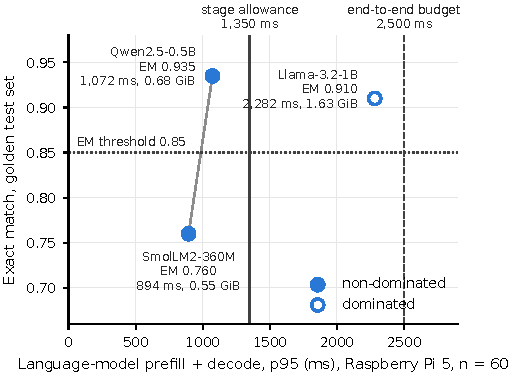
\includegraphics[width=\columnwidth]{figures/fig_pareto.pdf}
\caption{Golden-set EM against language-model p95 for the three \QF{} configurations on the cooled
Raspberry Pi~5; filled markers are non-dominated. Solid line: the 1,350~ms language-model
allowance, measured on the same quantity as the axis; dashed: the 2,500~ms end-to-end budget, of
which the axis measures only part; dotted: the 0.85 EM threshold. The \QE{} artefacts were not
timed and are not plotted.}
\label{fig:pareto}
\end{figure}

Figure~\ref{fig:pareto} places the three timed configurations against the constraints. No
configuration is shown to satisfy both constraints of the selection rule. The memory ceiling applies to
the full stack, which was not measured; the language-model process alone uses 0.55--1.63~GiB, about
35\% or more below the ceiling. The end-to-end budget was measured for Qwen2.5-0.5B only, by the
latency experiment of the companion paper~\citep{companion}: its p95 is 3,122~ms over 226 speech
segments, 622~ms (25\%) above the budget. The shortest speech-recognition time in that experiment
is 1,063~ms, so Llama-3.2-1B's end-to-end p95 is at least 3,346~ms. SmolLM2-360M was not measured
end to end.

Under the failure clause, the memory ceiling is applied to the language-model process, which every
configuration satisfies, and the end-to-end budget is re-baselined to the measured 3,122~ms, which
Llama-3.2-1B misses and SmolLM2-360M is not shown to meet. The rule selects Qwen2.5-0.5B at \QF{}.
Admitting SmolLM2-360M as well leaves the selection unchanged, because its EM of 0.760 is
significantly lower (Table~\ref{tab:mcnemar}). No \QE{} artefact exceeds 0.935. Qwen2.5-0.5B at
\QF{} is the only configuration that meets the EM, intent-F1, decode, throughput and throttling
targets and, with a cached prefix, the combined language-model allowance together; it misses the
250~ms prefill allowance. Qwen2.5-0.5B and SmolLM2-360M are non-dominated, and
Llama-3.2-1B is dominated on the point estimates.

% =============================================================================
\section{Discussion}
\label{sec:discussion}

\paragraph{Parameter count does not order these models.} The 0.49~B model is at least as accurate
as the 1.24~B model on the golden set. With only five discordant pairs, the smallest attainable
exact $p$ is 0.0625, so no split of them could have reached the corrected $\alpha$; the test could not
have established a difference, and its result does not establish equivalence. At matched size, the
family difference (6.5\pp{}) is more than 40\% of the span across the whole 3.4-fold size range (15.0\pp{}). For a narrow task in the
sub-1.5~B range, choosing a model by size alone would have selected a slower model with no
established accuracy gain. Two qualifications apply. Each family is represented by one model at
one size, so a family effect cannot be expressed as a share of a size effect. And the
three-epoch budget left most models short of convergence: the lower-scoring model of each contrast
gained most in validation EM at the last epoch (SmolLM2-360M by 0.025, H2O-Danube3-500M by 0.038),
so part of both gaps may reflect convergence speed rather than capacity. The comparison is one of
performance under an identical training budget. Within it, the trade-off has a measured price:
moving from Qwen2.5-0.5B to SmolLM2-360M saves 178~ms of p95 and 0.13~GiB of memory and costs
17.5\pp{} of EM, a significant difference.

\paragraph{What the grammar adds after fine-tuning.} Without the grammar, the fine-tuned models left
the format once in 3,540 decodes, and EM moved by 0.17\pp{} in the grammar's favour. The grammar's
measurable contribution to validity on these test sets is that single decode. Its main value,
however, is not a rate. Under the grammar, no output that violates the schema is reachable for any
input, and no finite test set can measure a property of that kind. The one failure fell on an
out-of-domain query, where the training distribution ends, which is where a guarantee matters.
Bounding the grammar mattered as much as having one. An unbounded identifier list caused the
truncation loop of Section~\ref{sec:intro}, and the bounded grammar makes it unreachable. The
documented costs of constrained decoding, distribution distortion~\citep{park2024} and lower
accuracy on reasoning tasks~\citep{tam2024}, do not appear in EM here. This is consistent with
the finding of \citet{tam2024} for classification-like tasks: a single-turn schema with ten intents is closer
to classification than to multi-step reasoning. Prior grammar studies used models that were not
fine-tuned to the format~\citep{geng2023,tam2024}. For a fine-tuned model, our data suggest the
grammar is cheap insurance rather than a source of accuracy.

\paragraph{Deployment cost in context.} The fp16-to-deployed delta is not comparable with the
isolated quantisation losses reported for larger models~\citep{kurtic2025,kurt2026}, because it
combines precision, runtime, grammar and decoding settings. What it establishes is narrower and
practical: on this task, the complete path from the trained model to the artefact that runs on the
board cost at most three golden items net, and \QF{} cost no established accuracy relative to
\QE{}. Since \QF{} is the only level timed on the board, a \QE{} deployment would need its own
timing before it could be selected.

\paragraph{Thermal state belongs in the benchmark.} Single-board benchmarks report throughput as a
property of a model and runtime~\citep{sbc2025}. Our data show that on the same board, with the
same artefact, Qwen2.5-0.5B clears the 20~tokens/s floor by 40\% with an active cooler and falls
below it without one. A throughput figure for such a board describes the enclosure as well as the
model, and should be reported with the throttle state it was measured under. The attribution to
clock speed is incomplete: the uncooled run was capped at, not held at, 1.5~GHz, and the clock
actually held was not logged. SmolLM2-360M's 1.69-fold throughput gain is explained by the clock
alone only if the throttled clock fell below 1.42~GHz.

\paragraph{Abstention is the main shortfall.} The models abstain on most out-of-domain inputs but
almost never on in-domain ones (once in 2,640 decodes), even when they are wrong. They appear to
have learned to classify request types rather than to signal uncertainty. This matters because a
misrecognised command still reads as a supported request, and nearly every in-domain error
(98.9\%) would dispatch an executable command. The dominant error, a sign error on the yaw angle,
illustrates why later validation layers cannot compensate: both signs are legal values, so nothing
within a single command distinguishes the intended direction from its opposite. One untested
explanation is that the schema encodes direction as a sign, so a spoken ``clockwise'' must become
a minus sign that the transcript never contains. The training data teach \texttt{unknown} through
81 out-of-scope utterances and through none in which a supported command is made unreadable. Two
remedies follow: a confidence gate that routes low-probability decodes to \texttt{unknown}, and
training pairs that map degraded commands to \texttt{unknown}. Neither was implemented here.

\paragraph{Limitations.} All accuracy figures are measured on reference transcripts, so they
overstate what the pipeline achieves from audio; the word error rate on the golden speaker is
23.3\% through the deployed pipeline~\citep{companion}. The golden set is one speaker in one session, and its 200 items are paraphrases
of 12 command patterns, so the effective sample is smaller than 200 and the intervals and
$p$-values are optimistic. The golden and synthetic test sets are drawn from the same 12 held-out
families, so agreement between them shows consistency on those patterns rather than two
independent confirmations. Labels are generated rather than independently annotated. Each model was trained once,
with one seed and a fixed budget; the control differs in system-prompt rendering and training
session, and GPU training is not bit-reproducible across sessions~\citep{pytorchrepro}. Timing comes
from one board and one runtime build, with a cached prefill. Only the selected configuration was
measured end to end, and the full-stack memory of no configuration was measured. Finally, the
schema is small: single-turn, ten intents and a bounded slot vocabulary. Whether the ordering of
models or the grammar's low cost carries over to richer schemas is not established.

% =============================================================================
\section{Conclusion}
\label{sec:conclusion}

Among three fine-tuned small language models quantised for CPU-only inference on a Raspberry~Pi~5,
Qwen2.5-0.5B at \QF{} offers the best accuracy--efficiency trade-off for grammar-constrained
command parsing: 0.935 golden-set EM at 27.93~tokens/s on a cooled board. On the golden set it is
at least as accurate as a model 2.5 times its size (0.910, a difference that is not significant),
and significantly more accurate than the smallest candidate. A bounded
grammar guarantees structural validity at no measured accuracy cost, and the deployment pipeline
from fp16 to the quantised artefact costs no established accuracy. Two results qualify the choice:
its end-to-end latency exceeds the 2,500~ms budget, and no configuration meets the false-command or
safe-failure targets. Future work will add a log-probability confidence gate and training pairs for
unreadable commands to address abstention, and will measure the smaller SmolLM2-360M end to end to
complete the frontier at its fast end.

% =============================================================================
\printcredits

\section*{Funding}
This research did not receive any specific grant from funding agencies in the public, commercial,
or not-for-profit sectors.

\section*{Declaration of competing interest}
The authors declare that they have no known competing financial interests or personal
relationships that could have appeared to influence the work reported in this paper.

\section*{Data availability}
The command schema and grammar, the dataset splits including the golden-set recordings, the
training configurations, the evaluation harness, the raw measurement files and the scripts that
produce every table and figure in this article are publicly available at
\url{https://github.com/TayebKahia/voice-swarm-edge-}. The deployed \QF{} artefact is distributed
through the repository's releases.

\section*{Declaration of generative AI and AI-assisted technologies in the writing process}
During the preparation of this work the authors used Claude (Anthropic) for writing assistance.
After using this tool, the authors reviewed and edited the content as needed and take full
responsibility for the content of the publication.

\bibliographystyle{cas-model2-names}
\bibliography{references}

\end{document}
